\documentclass[t,handout,aspectratio=169]{beamer}
%\documentclass[t,aspectratio=169]{beamer}
\usetheme[
    sectionpage=progressbar,
    subsectionpage=none,
    numbering=none,
    block=fill,
]{metropolis}

\usepackage[T1]{fontenc}
\usepackage[utf8]{inputenc}
% \usepackage[english,nswissgerman]{babel}
\usepackage[nswissgerman,english]{babel}
\usepackage{listings}
\lstset{ %
    basicstyle=\ttfamily\footnotesize,
    breaklines=true,
    columns=fullflexible,
    keepspaces=true,
    language=bash,
    tabsize=2
}

%%%%%%%%%%%%%%%%%%%%%%%%%%%%%%%%%%%%%%%%%%%%%%%%%%%%%%%%%%%%%%%%%%%%%%%%

\title{Taskwarrior}
\subtitle{Philosophy and Ecosystem}
\titlegraphic{\hfill
\includegraphics[height=3cm]{tw-xl.png}}

\date{December, 9th 2016}
\author{Dirk Deimeke}
\institute{Taskwarrior Academy @ TNG Technology Consulting GmbH}

\subject{Taskwarrior}
\keywords{Taskwarrior}

%%%%%%%%%%%%%%%%%%%%%%%%%%%%%%%%%%%%%%%%%%%%%%%%%%%%%%%%%%%%%%%%%%%%%%%%

\begin{document}

\begin{frame}
    \titlepage
\end{frame}

%%%%%%%%%%%%%%%%%%%%%%%%%%%%%%%%%%%%%%%%%%%%%%%%%%%%%%%%%%%%%%%%%%%%%%%%
\section{Prolog}
%%%%%%%%%%%%%%%%%%%%%%%%%%%%%%%%%%%%%%%%%%%%%%%%%%%%%%%%%%%%%%%%%%%%%%%%

%%%%%%%%%%%%%%%%%%%%%%%%%%%%%%%%%%%%
\subsection{Dirk Deimeke}
%%%%%%%%%%%%%%%%%%%%%%%%%%%%%%%%%%%%

\begin{frame}[standout]
    Dirk Deimeke -- \href{https://d5e.org/}{d5e.org}
\end{frame}

\begin{frame}[fragile]\frametitle{Very Simple Rules}
    \vfill \pause
    \begin{itemize}
        \item No ``Sie'' -- please use \textbf{``Du''}! \pause
        \item Questions? Ask!
    \end{itemize}
\end{frame}

%%%%%%%%%%%%%%%%%%%%%%%%%%%%%%%%%%%%
\subsection{The right tool}
%%%%%%%%%%%%%%%%%%%%%%%%%%%%%%%%%%%%

\begin{frame}[standout]
    The right tool.
\end{frame}

\begin{frame}[standout]
    The right tool is reliable.
\end{frame}

\begin{frame}[standout]
    The right tool is methodology agnostic.
\end{frame}

\begin{frame}[standout]
    The right tool does not stand in your way.
\end{frame}

\begin{frame}[standout]
    The right tool for task management \pause \\
    helps you focus on only a few tasks to do.
\end{frame}

\begin{frame}[standout]
    The right tool is the tool you \underline{want} to use.
\end{frame}

%%%%%%%%%%%%%%%%%%%%%%%%%%%%%%%%%%%%%%%%%%%%%%%%%%%%%%%%%%%%%%%%%%%%%%%%
\section{Taskwarrior}
%%%%%%%%%%%%%%%%%%%%%%%%%%%%%%%%%%%%%%%%%%%%%%%%%%%%%%%%%%%%%%%%%%%%%%%%

%%%%%%%%%%%%%%%%%%%%%%%%%%%%%%%%%%%%
\subsection{Example}
%%%%%%%%%%%%%%%%%%%%%%%%%%%%%%%%%%%%

\begin{frame}[fragile]\frametitle{It is as easy as this example \ldots}
    \vfill
    \begin{lstlisting}
> task add Prepare Talk\end{lstlisting} \pause

\begin{lstlisting}
> task list\end{lstlisting} \pause

\begin{lstlisting}
> task 1 done\end{lstlisting}
\end{frame}

\begin{frame}[fragile]\frametitle{But it can be more \ldots}
    \vfill
    \begin{columns}[t]

        \begin{column}{0.45\textwidth}
            \begin{lstlisting}
> task add \
    project:private.birthdays \
    +anniversary \
    due:2017-01-11T10:00:00Z \
    scheduled:2016-12-24 \
    wait:soq \
    until:due+7days \
    Send birthday card to Alice\end{lstlisting} \pause
        \end{column}

        \begin{column}{0.45\textwidth}
            \begin{lstlisting}
> task add \
    project:tngtech.administration \
    due:eom \
    priority:M \
    +boring \
    +important \
    recurr:monthly \
    Prepare Meeting\end{lstlisting} \pause
        \end{column}

    \end{columns}

    \begin{center}
        \textbf{More sophisticated usage in the workshop this afternoon.}
    \end{center}
\end{frame}

%%%%%%%%%%%%%%%%%%%%%%%%%%%%%%%%%%%%
\subsection{Background}
%%%%%%%%%%%%%%%%%%%%%%%%%%%%%%%%%%%%

\begin{frame}[fragile]\frametitle{Background}
    \vfill
    Project founder Paul Beckingham:

    \begin{quote}
        I started out using Gina Trapani's todo.sh, which was great, \\
        but I soon wanted features that would have been difficult \\
        to implement in a shell script, so I wrote my own.
    \end{quote}
\end{frame}

%%%%%%%%%%%%%%%%%%%%%%%%%%%%%%%%%%%%
\subsection{Motivation}
%%%%%%%%%%%%%%%%%%%%%%%%%%%%%%%%%%%%

\begin{frame}[fragile]\frametitle{Motivation}
    \vfill
    Project founder Paul Beckingham:

    \begin{quote}
        It stemmed from the fact that a todo program needs to be \\
        simple to use, and unobtrusive, otherwise it's a hassle. \pause

        \textbf{But it can't be too simple.}
    \end{quote}
\end{frame}

%%%%%%%%%%%%%%%%%%%%%%%%%%%%%%%%%%%%
\subsection{History}
%%%%%%%%%%%%%%%%%%%%%%%%%%%%%%%%%%%%

\begin{frame}[fragile]\frametitle{History -- Some milestones}
    \vfill
    \begin{description}
        \item[2006-11-29, v0.0.1]  \hfill \\
            Project began as enhancement to todo.txt.
        \item[2014-01-15, v2.3.0]  \hfill \\
            Task Server support.
        \item[2015-10-21, v2.5.0]  \hfill \\
            Improved command line parser.
        \item[2016-02-24, v2.5.1]  \hfill \\
            bug fix, code cleanup, performance release -- no features.
        \item[near future, v2.6.0] \hfill \\
            overhaul recurrence and add more flavors of recurring tasks.
    \end{description}
    \url{https://taskwarrior.org/docs/history.html}
\end{frame}

%%%%%%%%%%%%%%%%%%%%%%%%%%%%%%%%%%%%
\subsection{Philosophy}
%%%%%%%%%%%%%%%%%%%%%%%%%%%%%%%%%%%%

\begin{frame}[standout]
    Taskwarrior is developed using a philosophy \\
    that explains a lot about why certain decisions \\
    have been made, and will continue to be made.
\end{frame}

\begin{frame}[fragile]\frametitle{Openness}
    \vfill
    The source code, plans, bugs, testing, docs, website are all free and open source. \pause

    Your data is kept as plain text, and never held hostage by a proprietary format.
\end{frame}

\begin{frame}[fragile]\frametitle{Low Friction}
    \vfill
    There should be no login authentication, lengthy launch, or interactivity \\
    getting in the way of simply capturing information.
\end{frame}

\begin{frame}[fragile]\frametitle{No Penalty}
    \vfill
    There should be no penalty for features that exist, but you don't use. \pause

    But that also means the features are there if you need them.
\end{frame}

\begin{frame}[fragile]\frametitle{Methodology Agnostic}
    \vfill
    While methodologies are important, Taskwarrior doesn't impose or prefer any methodology, and instead acknowledges that everyone works differently, placing different emphasis on things like priorities, due dates, dependence and so on.
\end{frame}

\begin{frame}[fragile]\frametitle{Toolkit}
    \vfill
    Supporting all methodologies and workflows means there are a lot of features, but you are not expected to use them all. \pause

    Think of Taskwarrior as a toolkit that lets you follow any methodology you choose, and any methodology will only use a subset of the features.
\end{frame}

\begin{frame}[standout]
    There is a fine line between \\
    ``richly-featured'' and ``bloated''.

    There may not be a line at all.
\end{frame}

\begin{frame}[fragile]\frametitle{Extension Friendly}
    \vfill
    Import/export using industry-standard JSON allows you to move data into and out of Taskwarrior, so you can provide a front end, or higher-order feature.
\end{frame}

\begin{frame}[fragile]\frametitle{Focus}
    \vfill
    Taskwarrior carefully limits the features it supports, in order to focus on doing one thing well. \pause

    It does not offer reminders and time tracking, because there is other software dedicated to implementing those features well. \pause

    \textbf{If a feature improves the way we manage task lists, then it belongs in Taskwarrior, otherwise it belongs in some other software.}
\end{frame}

\begin{frame}[standout]
    What you keep out of a project \\
    is just as important as \\
    what you allow in to a project.
\end{frame}

%%%%%%%%%%%%%%%%%%%%%%%%%%%%%%%%%%%%
\subsection{Documentation}
%%%%%%%%%%%%%%%%%%%%%%%%%%%%%%%%%%%%

\begin{frame}[fragile]{Documentation}
    \vfill
    \begin{quote}
        Everybody wants it, \\
        noone wants to write it, \\
        most of the people don't read it \ldots
    \end{quote}
\end{frame}

\begin{frame}[fragile]\frametitle{Website -- \url{https://taskwarrior.org/docs/}}
    \begin{center}
        \href{https://taskwarrior.org/docs/}{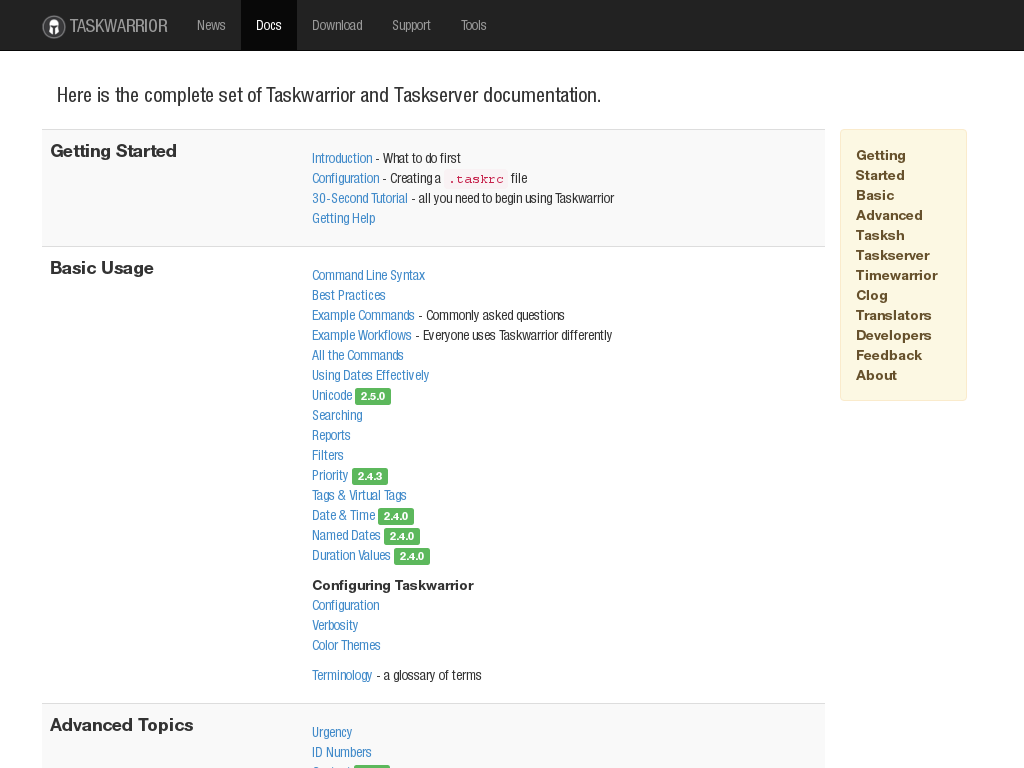
\includegraphics[height=7cm]{taskwarrior-org-docs.png}}
    \end{center}
\end{frame}

\begin{frame}[fragile]\frametitle{manpages}
    \vfill
    \begin{lstlisting}
> man task       # 1187 lines

> man taskrc     # 1182 lines
> man task-color #  330 lines
> man task-sync  #  164 lines

# total:           2863 lines of information
#                  (close to 50 printed pages)\end{lstlisting}
\end{frame}

\begin{frame}[fragile]\frametitle{\texttt{task help}}
    \vfill
    \begin{lstlisting}
> task help

Usage: task                       Runs rc.default.command, if specified.
       task <filter> active       Active tasks
       task          add <mods>   Adds a new task
       task <filter> all          All tasks
...

# 241 lines of adhoc-help\end{lstlisting}
\end{frame}

\begin{frame}[fragile]\frametitle{Guides -- easier to read}
    \vfill
    Lesson learned:
    \begin{quote}
        Man pages are too densely crammed with information, \\
        and too lengthy, for most modern humans to ingest.
    \end{quote} \pause
    We offer PDF guides and presentations: \\
    \url{https://git.tasktools.org/projects/ST/repos/guides/browse}
\end{frame}

%%%%%%%%%%%%%%%%%%%%%%%%%%%%%%%%%%%%
\subsection{Taskserver}
%%%%%%%%%%%%%%%%%%%%%%%%%%%%%%%%%%%%

\begin{frame}[fragile]\frametitle{The need!}
    \vfill
    With people running Taskwarrior on several machine the need rises to sync the task data between machines.
\end{frame}

\begin{frame}[standout]
    Taskserver synchronises Taskwarrior data.
\end{frame}

\begin{frame}[fragile]\frametitle{Why Do I Need a Taskserver?}
    \vfill
    You may not need a Taskserver. \pause

    You may be content with using Taskwarrior on a single device. \pause

    But if you wish to share tasks between several clients, \\
    the Taskserver is the \textbf{only} option that properly syncs data.
\end{frame}

\begin{frame}[fragile]\frametitle{One feature does it all}
    \vfill
    With a Taskserver, you can share tasks between clients/devices, \\ \pause
    eliminating the need to keep your data up to date on multiple clients, \\ \pause
    reducing data entry. \pause

    One nice side effect of using a Taskserver is an automatic backup of your tasks.
\end{frame}

\begin{frame}[fragile]\frametitle{Short history, long time}
    \vfill
    \begin{description}
        \item[2010-09-22]  \hfill \\
            Project began.
        \item[2012-09-26]  \hfill \\
            Project restarted using GnuTLS.
        \item[2014-01-15, v1.0.0]  \hfill \\
            Sync Protocol v1. Compatibility with Taskwarrior 2.3.0.
        \item[2015-05-10, v1.1.0]  \hfill \\
            Improved security, logging, portability, documentation, quality, setup, PKI scripts. IPv4/IPv6 support. Many bug fixes.

            Short: Everything is better now.
    \end{description}
    \url{https://taskwarrior.org/docs/history_td.html}
\end{frame}

%%%%%%%%%%%%%%%%%%%%%%%%%%%%%%%%%%%%
\subsection{Timewarrior}
%%%%%%%%%%%%%%%%%%%%%%%%%%%%%%%%%%%%

\begin{frame}[fragile]\frametitle{Time tracking}
    \vfill
    People -- at least some -- like to use Taskwarrior for time tracking. \pause

    This does not match our philosophy ``improves the way we manage task lists'', \\
    so it has to be another software.
\end{frame}

\begin{frame}[standout]
    Timewarrior tracks and reports time.
\end{frame}

\begin{frame}[fragile]\frametitle{What does Timewarrior do?}
    \vfill
    Timewarrior is a command line time tracking application, \\
    which allows you to record time spent on activities. \pause

    At its simplest, you tell it to start and stop tracking time:

    \begin{lstlisting}
> timew start
...
> timew stop\end{lstlisting}
\end{frame}

\begin{frame}[fragile]\frametitle{Why do I need Timewarrior?}
    \vfill
    You will be able to track your time intelligently, \\
    then generate useful visual or tabular reports of that time. \pause

    An extension API lets you do anything you want with your data.
\end{frame}

\begin{frame}[fragile]\frametitle{Example}
    \vfill
    Suppose you start the clock at noon on a Friday, \\
    then you stop the clock at noon on Tuesday. \pause

    Did you really just spend 96 hours on a task? \\ \pause
    More likely you only spent 16 hours, \\ \pause
    or perhaps 8 hours if Monday was a national holiday. \pause

    Timewarrior supports you in solving that riddle.
\end{frame}

\begin{frame}[fragile]\frametitle{How does Timewarrior work?}
    \vfill
    Timewarrior records time, and associates blocks of time with tags. \pause

    The recorded data can be exposed as JSON for any app to consume. \pause

    Built-in reports, as well as a set of extension reports will give you plenty of options. \pause

    A Taskwarrior hook script provides integration \\
    with the matching \verb=start= and \verb=stop= commands, \\
    thereby enabling proper time tracking for Taskwarrior users.
\end{frame}

\begin{frame}[fragile]\frametitle{History}
    \vfill
    \begin{description}
        \item[2016-08-21, v1.0.0]  \hfill \\
            Project released the time it was presented at FrOSCon.
    \end{description}
\end{frame}

%%%%%%%%%%%%%%%%%%%%%%%%%%%%%%%%%%%%%%%%%%%%%%%%%%%%%%%%%%%%%%%%%%%%%%%%
\section{Ecosystem}
%%%%%%%%%%%%%%%%%%%%%%%%%%%%%%%%%%%%%%%%%%%%%%%%%%%%%%%%%%%%%%%%%%%%%%%%

%%%%%%%%%%%%%%%%%%%%%%%%%%%%%%%%%%%%
\subsection{Additions}
%%%%%%%%%%%%%%%%%%%%%%%%%%%%%%%%%%%%

\begin{frame}[fragile]\frametitle{Tasktools -- \url{https://tasktools.org/}}
    \begin{center}
        \href{https://tasktools.org/}{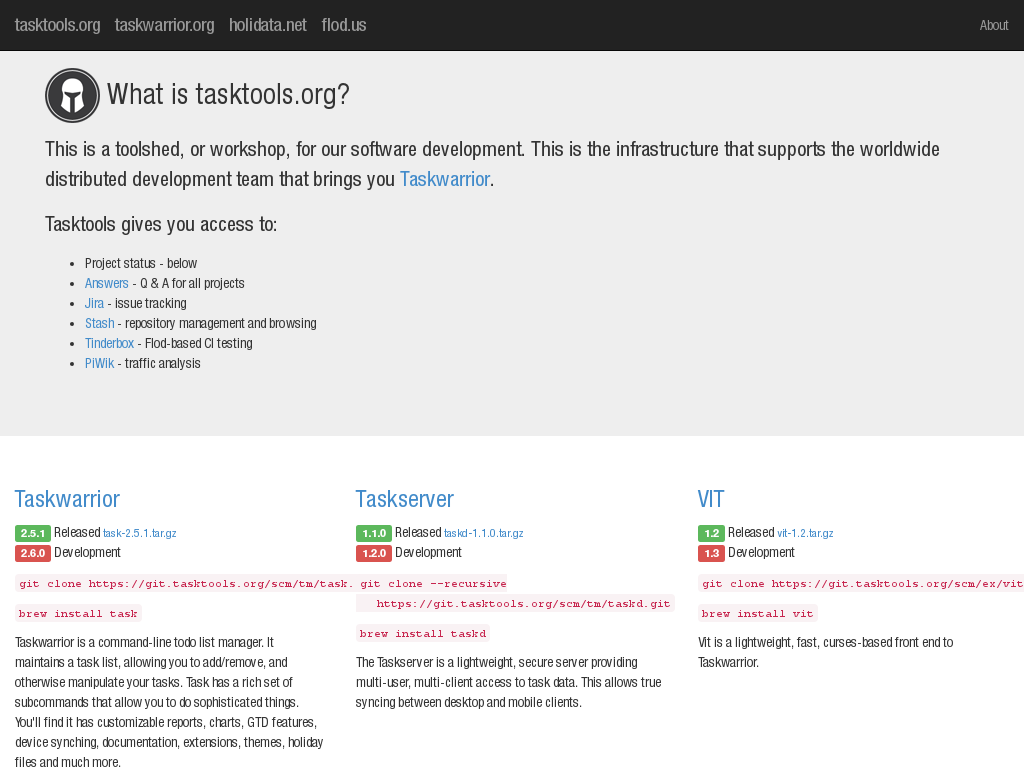
\includegraphics[height=7cm]{tasktools-org.png}}
    \end{center}
\end{frame}

\begin{frame}[fragile]\frametitle{tasksh -- \url{https://tasktools.org/projects/tasksh.html}}
    \vfill
    Tasksh is a shell command that wraps Taskwarrior commands. It is intended to provide simpler Taskwarrior access.

    Tasksh implements a review feature, and integrates libreadline. It is on it's own release schedule that is unhampered by lengthy Taskwarrior development cycles.

    Future Tasksh releases are being planned now. Features currently being designed include:
    \begin{itemize}
        \item Pomodoro Timer
        \item Notifications
    \end{itemize}
\end{frame}

\begin{frame}[fragile]\frametitle{3rd Party Apps -- \url{https://taskwarrior.org/tools/}}
    \begin{center}
        \href{https://taskwarrior.org/tools/}{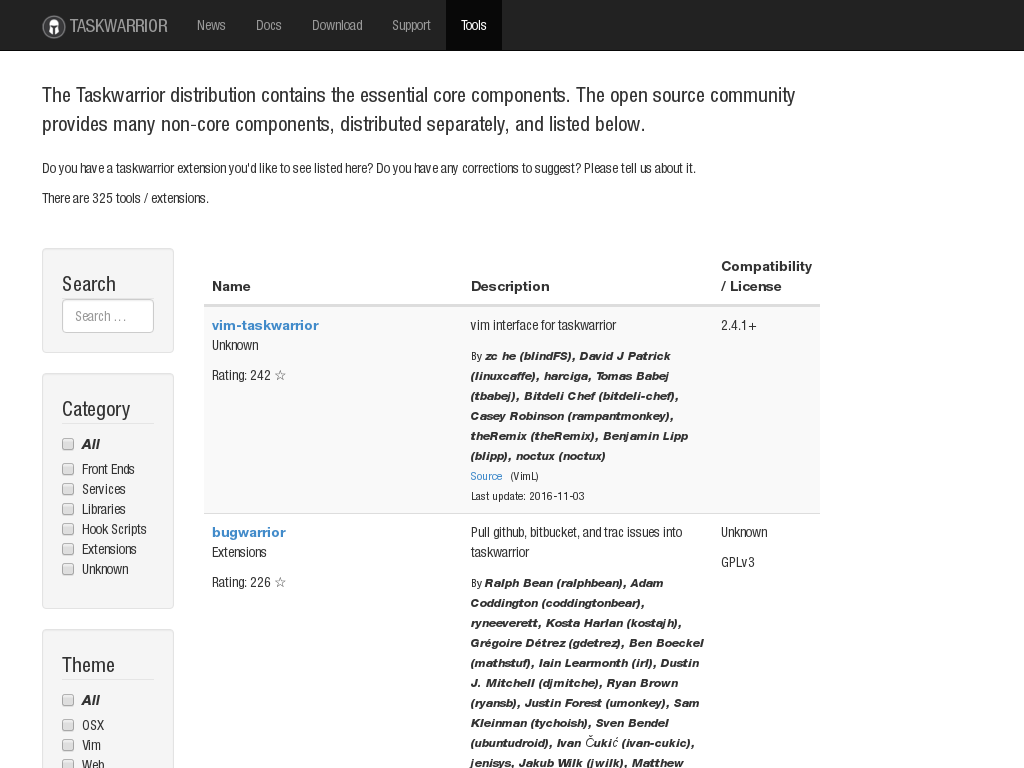
\includegraphics[height=7cm]{3rdparty.png}}
    \end{center}
\end{frame}

\begin{frame}[fragile]\frametitle{taskopen -- \url{https://github.com/ValiValpas/taskopen}}
    \vfill
    Taskopen allows you to link almost any file, webpage or command to a Taskwarrior task by adding a filepath, web-link or uri as an annotation.

    Text notes, images, PDF files, web addresses, spreadsheets and many other types of links can then be filtered, listed and opened by using taskopen.

    Some actions are sane defaults, others can be custom-configured, and everything else will use your systems mime-types to open the link.

    Arbitrary commands can be used with taskopen at the CLI, acting on the link targets, enhancing listings and even executing annotations as commands.
\end{frame}

\begin{frame}[fragile]\frametitle{vit -- \url{https://tasktools.org/projects/vit.html}}
    \vfill
    VIT (Visual Interactive Taskwarrior) is a lightweight, curses-based front end for Taskwarrior that provides a convenient way to quickly navigate and process tasks.

    VIT allows you to interact with tasks in a Vi-intuitive way.

    A goal of VIT is to allow you to customize the way in which you use Taskwarrior's core commands as well as to provide a framework for easily dispatching external commands (both user scripts and Taskwarrior's many External Scripts).
\end{frame}

\begin{frame}[fragile]\frametitle{Android -- \url{https://bitbucket.org/kvorobyev/taskwarriorandroid/}}
    \vfill
    \begin{itemize}
        \item Because Android application uses task binary for all manipulations with tasks, in general, you can expect exactly same behaviour with original Taskwarrior
        \item Synchronisation with taskd server works!
        \item Features below are unique to Android version:
        \begin{itemize}
            \item Create shortcuts to reports and new task templates to Home screen
            \item Multiple profiles support
            \item Auto-syncronisation by configurable intervals
        \end{itemize}
        \item Following features are not implemented at present moment:
        \begin{itemize}
            \item UDAs
            \item Dependencies
        \end{itemize}
    \end{itemize}
    \url{https://play.google.com/store/apps/details?id=kvj.taskw}
\end{frame}

\begin{frame}[fragile]\frametitle{GUI Client -- \url{https://bitbucket.org/kvorobyev/taskwarriorc2}}
    \vfill
    \begin{center}
        \href{https://bitbucket.org/kvorobyev/taskwarriorc2}{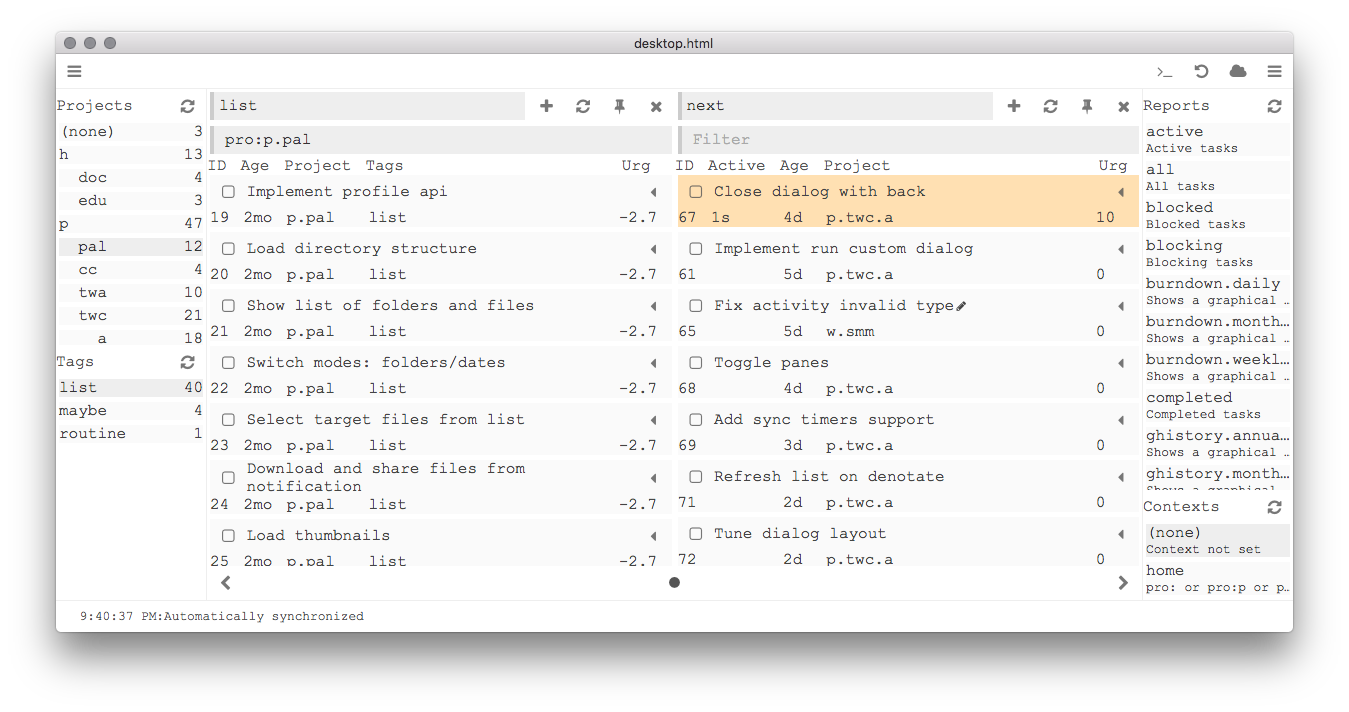
\includegraphics[height=5cm]{taskwarriorc2.png}}
    \end{center}
    Linux, macOS and Android,
    \url{https://play.google.com/store/apps/details?id=com.taskwc2}
\end{frame}

%%%%%%%%%%%%%%%%%%%%%%%%%%%%%%%%%%%%
\subsection{Other websites}
%%%%%%%%%%%%%%%%%%%%%%%%%%%%%%%%%%%%

\begin{frame}[fragile]\frametitle{Contribute to Taskwarrior}
    \vfill
    Want to contribute? -- \url{https://taskwarrior.org/docs/contribute.html}
    \vfill
	\begin{alertblock}{How to become an Open Source Contributor}
		We have some information for you on how to become an Open Source Contributor for the first time (\url{http://taskwarrior.org/docs/first_time.html} -- applies to the second and third contribution as well).
	\end{alertblock}
\end{frame}

\begin{frame}[fragile]\frametitle{Questions and Answers -- \url{https://answers.tasktools.org/}}
    \begin{center}
        \href{http://answers.tasktools.org/}{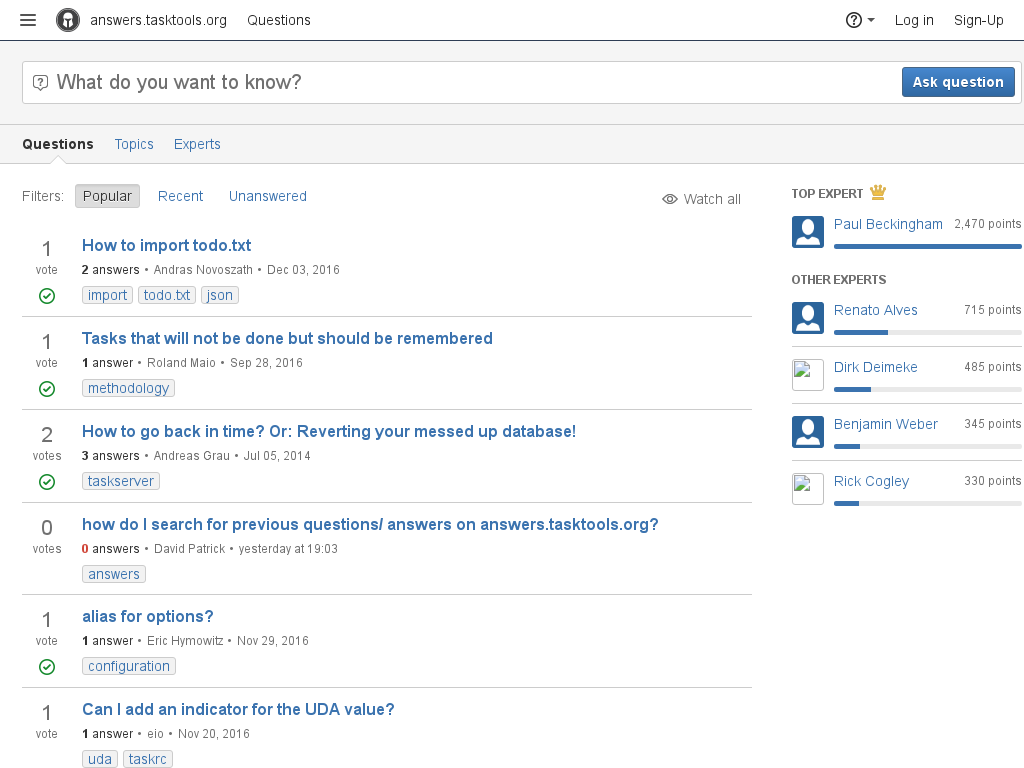
\includegraphics[height=7cm]{answers-tasktools-org.png}}
    \end{center}
\end{frame}

\begin{frame}[fragile]\frametitle{Issue Tracking -- \url{https://bug.tasktools.org/}}
    \begin{center}
        \href{https://bug.tasktools.org/}{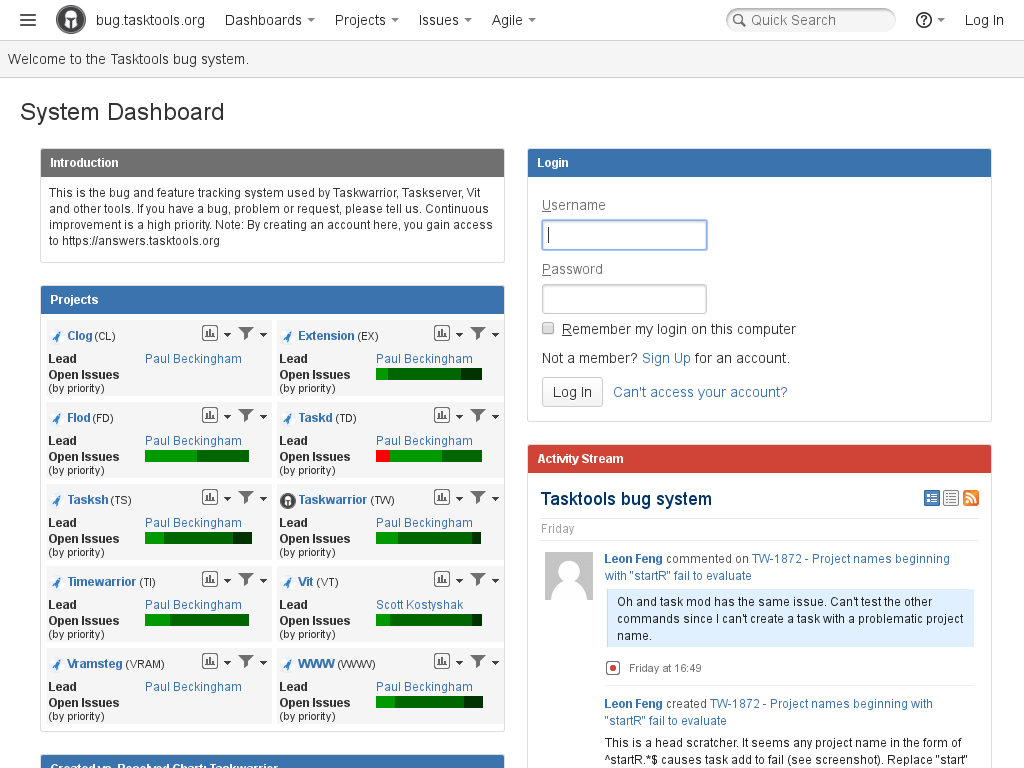
\includegraphics[height=7cm]{bug-tasktools-org.png}}
    \end{center}
\end{frame}

\begin{frame}[fragile]\frametitle{Repository Management -- \url{https://git.tasktools.org/}}
    \begin{center}
        \href{https://git.tasktools.org/}{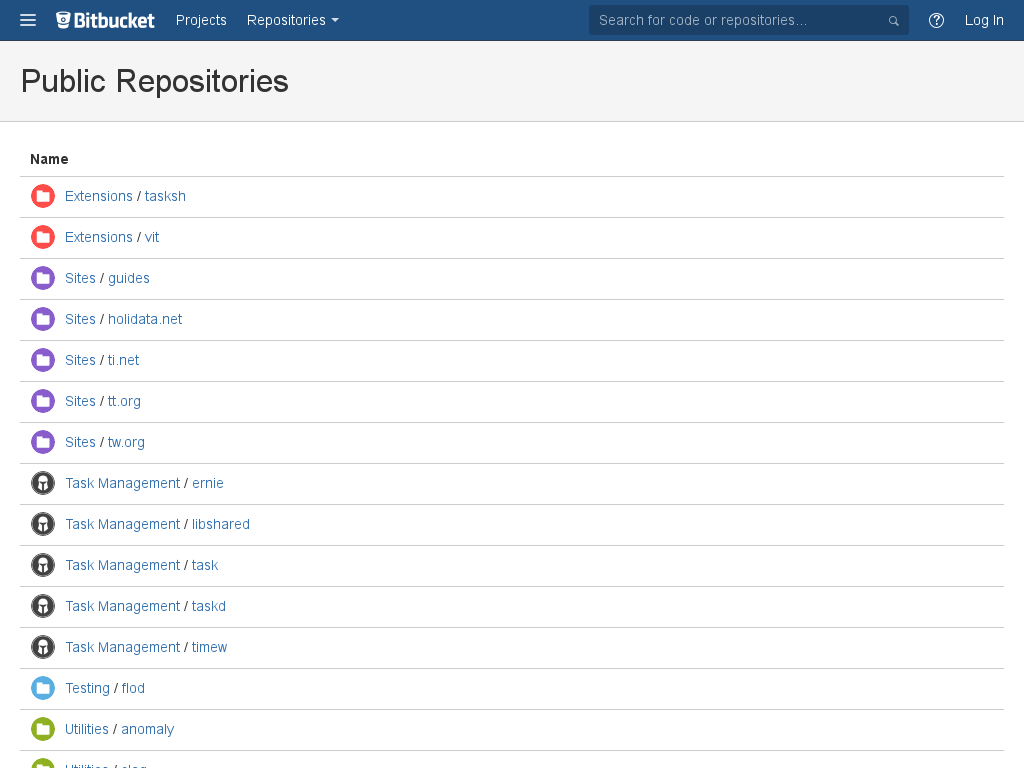
\includegraphics[height=7cm]{git-tasktools-org.png}}
    \end{center}
\end{frame}

\begin{frame}[fragile]\frametitle{Continous Integration -- \url{http://central.tasktools.org}}
    \begin{center}
        \href{http://central.tasktools.org/}{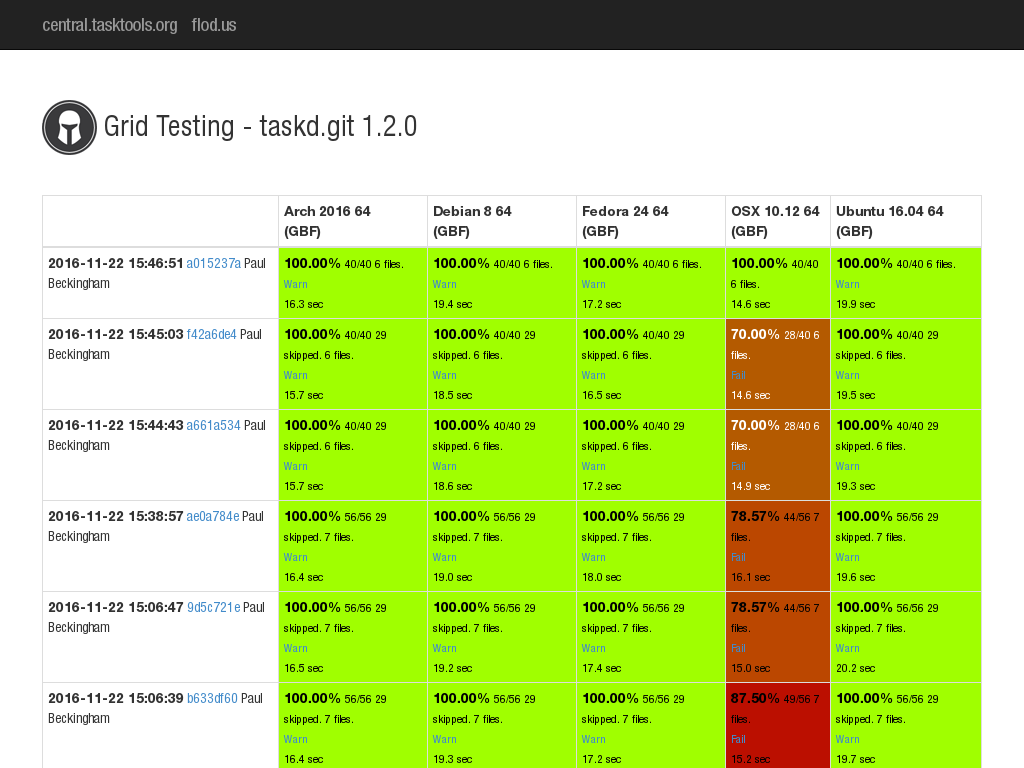
\includegraphics[height=7cm]{central-tasktools-org.png}}
    \end{center}
\end{frame}

\begin{frame}[fragile]\frametitle{IRC channel logger -- \url{https://botbot.me/freenode/taskwarrior/}}
    \begin{center}
        \href{https://botbot.me/freenode/taskwarrior/}{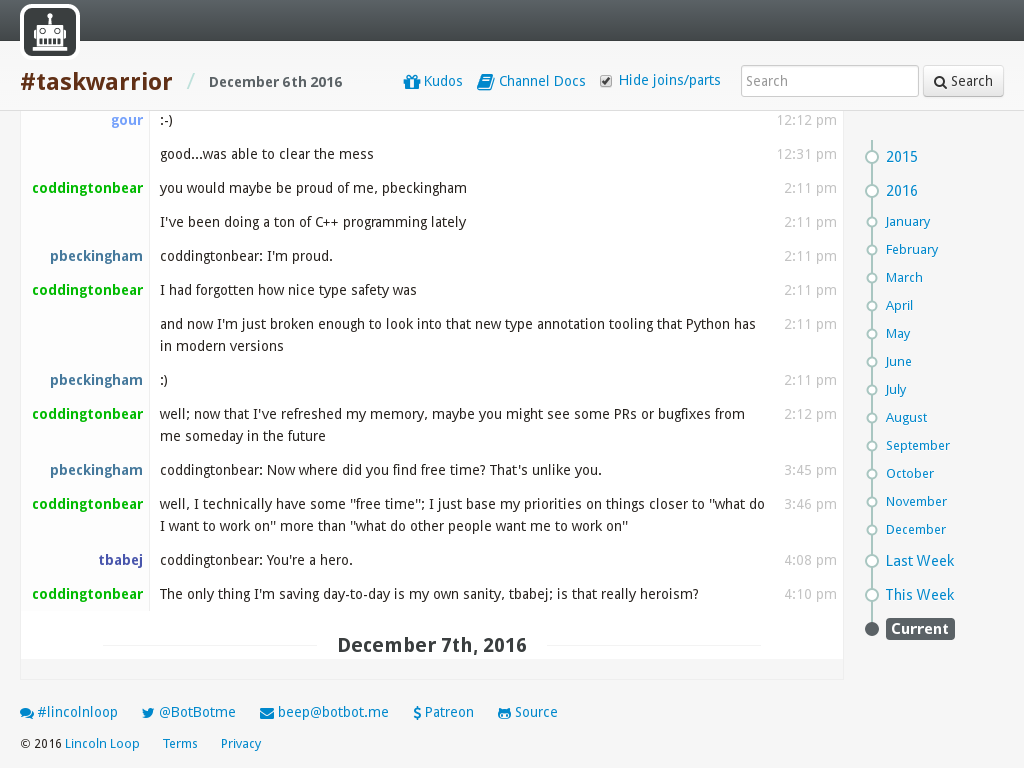
\includegraphics[height=7cm]{botbot-me-taskwarrior.png}}
    \end{center}
\end{frame}

%%%%%%%%%%%%%%%%%%%%%%%%%%%%%%%%%%%%
\subsection{Support}
%%%%%%%%%%%%%%%%%%%%%%%%%%%%%%%%%%%%

\begin{frame}[fragile]\frametitle{Getting Help}
    \vfill
    There are several ways of getting help:

    \begin{itemize}
        \item Submit your details to our \href{https://answers.tasktools.org}{\textbf{Q \& A site}}, then wait patiently for the community to respond.
        \item \textbf{Email} us at \href{mailto:support@taskwarrior.org}{support@taskwarrior.org}, then wait patiently for a volunteer to respond.
        \item Join us \textbf{IRC} in the \#taskwarrior channel on Freenode.net, and get a quick response from the community.
        \item Even though \textbf{Twitter} is no means of support, you can get in touch with \href{https://twitter.com/taskwarrior}{@taskwarrior}.
        \item We have a \href{https://groups.google.com/forum/\#!forum/taskwarrior-user}{\textbf{User Mailinglist}} which you can join anytime to discuss about Taskwarrior and techniques.
        \item The \href{https://groups.google.com/forum/\#!forum/taskwarrior-dev}{\textbf{Developer Mailinglist}} is focussing on a more technical oriented audience.
    \end{itemize}
\end{frame}

%%%%%%%%%%%%%%%%%%%%%%%%%%%%%%%%%%%%%%%%%%%%%%%%%%%%%%%%%%%%%%%%%%%%%%%%
\section{Epilog}
%%%%%%%%%%%%%%%%%%%%%%%%%%%%%%%%%%%%%%%%%%%%%%%%%%%%%%%%%%%%%%%%%%%%%%%%

\begin{frame}[fragile]\frametitle{Taskwarrior is platform independent}
    \vfill
    \begin{itemize}
        \item Most flavours of Unix and Linux, including macOS
        \item Windows 10 Linux Subsystem \\
            {\small (Other Windows versions with Cygwin -- unsupported, but known to work)}
        \item Android with Termux
        \item Third-Party Apps (Android-Client, GUI based on NodeJS, \ldots)
    \end{itemize}
\end{frame}

\begin{frame}[fragile]\frametitle{Conclusion}
    \vfill
    Taskwarrior \ldots \pause

    \ldots is easy to learn. \\ \pause
    \ldots grows along with the work. \\ \pause
    \ldots is unbelievably powerful. \\ \pause
    \ldots is very fast. \\ \pause
    \ldots is easily extensible. \\ \pause
    \ldots is actively developed. \\ \pause
    \ldots can be influenced by users (feature requests). \\ \pause
    \ldots has excellent and very friendly support.
\end{frame}

\begin{frame}[fragile]
    \vfill
    \begin{center}
        
\includegraphics[width=6.4cm,height=7cm]{task_logo.png}
    \end{center}
\end{frame}

\begin{frame}[fragile]\frametitle{Thank you!}
    \vfill
    \begin{center}
        Dirk Deimeke, 2016, \href{https://creativecommons.org/licenses/by/4.0/}{CC-BY}

        \href{mailto:dirk@deimeke.net}{dirk@deimeke.net}

        \href{https://d5e.org/}{d5e.org} -- \href{https://speakerdeck.com/ddeimeke/}{speakerdeck.com/ddeimeke} \\
        {\tiny Download the PDF for clickable links.}
    \end{center}
\end{frame}

\end{document}
